\section{Hardware design}

% HW design
Generelt kan det overordnede hardware design beskrives som noget elektronik der sender information ud på nettet, som sendes og analyseres af noget elektronik i den anden ende. Disse vil blive beskrevet herunder som encoder og decoder\footnote{For yderlige beregninger se projektdokumentation afsnit HW-design}.  


\section{Encoder}
Encoderen, også omtalt som senderenhed, er den del af systemet der genererer X10 kommandoen og sender den ud på det eksisterende el-net. Et højpasfilter der lader 120 kHz burst passere mens det blokerer for nettets 50 Hz signal, udgør sammen med en zero crossing detector hele hardwaren for encoderen.

\begin{figure}[htbp]
	\centering
	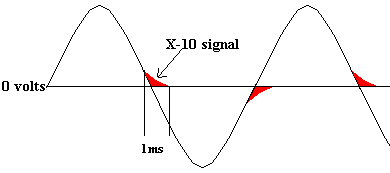
\includegraphics[width=0.50\textwidth]{billeder/HWdesign/X10_BURST}
	\caption{120 kHz burst i zero crossing}
	\label{fig:X10_BURST}
\end{figure}

Ideen med at sende burst ud på nettet i zero crossing kan ses illustreret på figur \ref{fig:X10_BURST}

\begin{figure}[htbp]
	\centering
	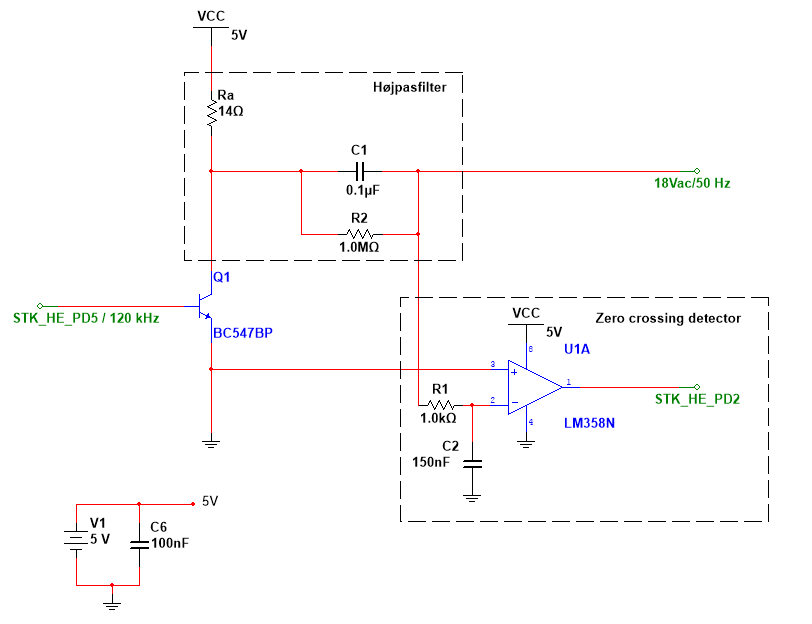
\includegraphics[width=0.70\textwidth]{billeder/HWdesign/Encoder}
	\caption{Samlet Encoder}
	\label{fig:Encoder}
\end{figure}
\newpage

\subsection{Højpasfilter}

\begin{figure}[htb]
  \begin{minipage}{0.45\textwidth}
    \centering
      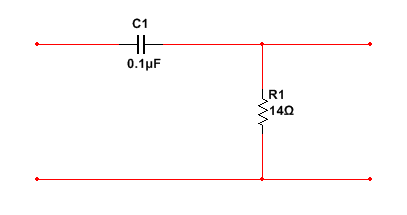
\includegraphics[width=\textwidth]{billeder/HWdesign/HP_MV}
      \caption{Højpasfilter med værdier}
    \label{fig:HP_MV}
  \end{minipage}
  \hspace{0.1\textwidth}
  \begin{minipage}{0.45\textwidth}
    \centering
      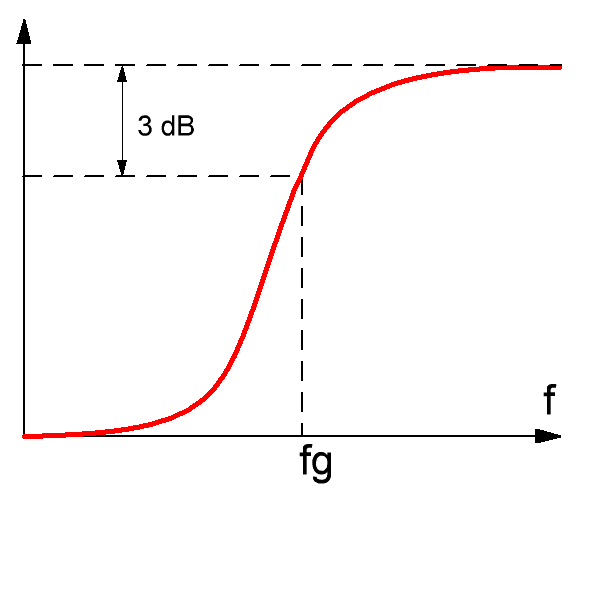
\includegraphics[width=\textwidth]{billeder/HWdesign/HP_KURVE}
      \caption{Kurvekarakteristik for højpasfilter}
    \label{fig:HP_KURVE}
  \end{minipage}
\end{figure}

For at sende X10 kommandoer ud på det eksisterende 50 Hz el-net er det nødvendigt at koble elektronikken direkte herpå og eftersom det elektronik ikke tåler de høje spændinger fra nettet, er det nødvendigt at blokere det signal, men stadig at kunne sende de 120 kHz ud. Dette løses med et højpasfilter.

Den ønskede knækfrekvens skal ligge omkring de 120 kHz for at opnå mindst dæmpning herpå. Ved denne knækfrekvens skulle 50 Hz signalet være ubetydelig lille efter filteret. 

Kondensatoren forudbestemmes for beregningerne til en værdi på 0,1 nF.


\newpage
  
\subsection{Zero Crossing Detector}
\begin{figure}[htb]
  \begin{minipage}{0.45\textwidth}
    \centering
      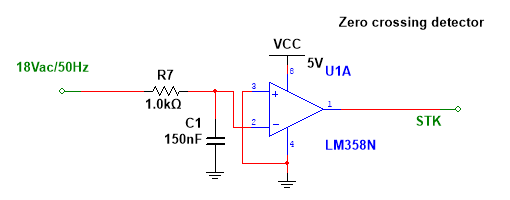
\includegraphics[width=\textwidth]{billeder/HWdesign/ZC_MV}
      \caption{Zero crossing detector med værdier}
    \label{fig:ZC_MV}
  \end{minipage}
  \hspace{0.1\textwidth}
  \begin{minipage}{0.45\textwidth}
    \centering
      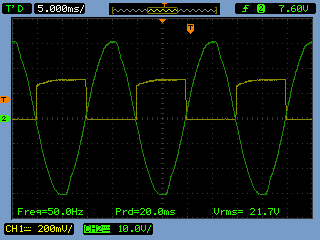
\includegraphics[width=\textwidth]{billeder/HWTest/Encoder/Encoder_zerocross}
      \caption{Scope billede af Zero crossing detector, CH1(indgangssignal), CH2(Udgangssignal)}
    \label{fig:Encoder_Zerocross}
  \end{minipage}
\end{figure}

Zero crossing detectoren har til opgave at detektere nulgennemgang, det er et krav for at X10 protokollen kan virke. Der er placeret en Zero crossing detector både på Encoderen og Decoderen, da begge disse består af et STK-kit der kræver information om nulgennemgang. Opbygning kan ses på overstående figur \ref{fig:ZC_UV}, der er anvendt en operationsforstærker af typen LM358N, som toggler udgangssignalet ved hver nulgennemgang se figur \ref{fig:Encoder_Zerocross}. Operationsforstærkerens positive ben er koblet til stel for at lave et triggerniveau til 0 V.

Modstanden $R_7$ sidder der bl.a. for at beskytte Zero crossing detectoren mod 18 VAC nettet, men sammen med kondensatoren udgør den også et lavpasfilter. Under implementeringen kunne det konstateres at der kom støj ind på Zero crossing detectoren, og dette problem løste lavpasfilteret. 

Der ønskes at dæmpe 120 kHz signalet, derfor designes lavpasfilteret ud fra en knækfrekvens på 1,0 kHz.

\section{Decoder}
Decoderen, som er den del i systemet der omdanner burst fra encoderen til X10 kommando, er opbygget af et båndpasfilter, zero crossing detector og en envelope detector. I starten af kredsløbet sidder båndpasfilteret, og dette blokerer for 50 Hz nettet og forstærker 120 kHz signalet der kommer fra encoderen. Herefter ledes signalet gennem envelope detector som omdanner burstet til et TTL signal.

\begin{figure}[htbp]
	\centering
	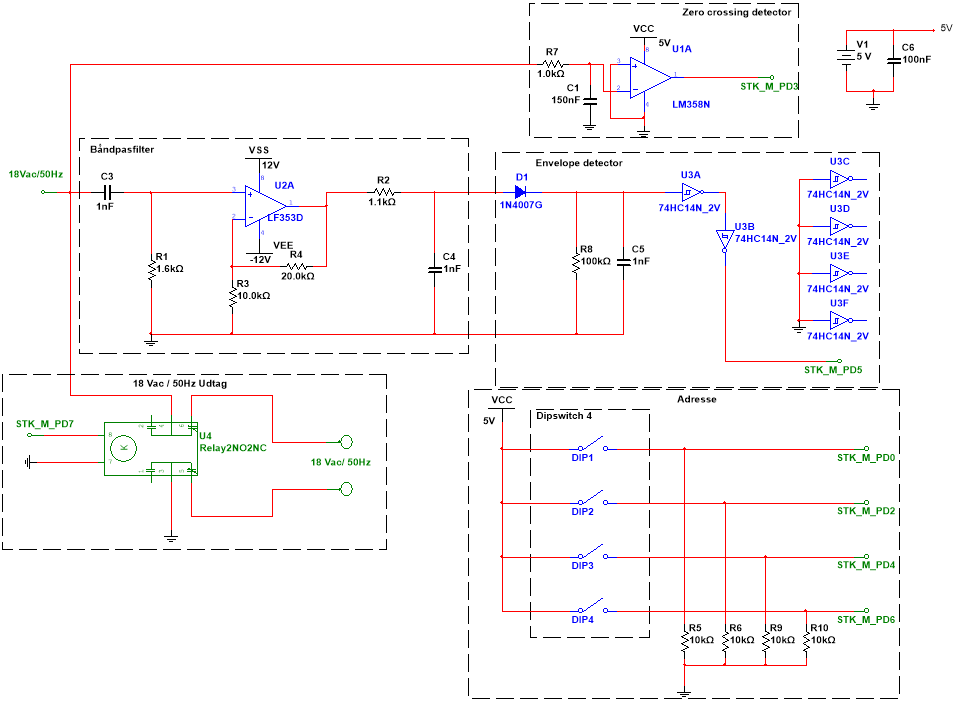
\includegraphics[width=0.70\textwidth]{billeder/HWdesign/Decoder}
	\caption{Samlet Decoder}
	\label{fig:Decoder}
\end{figure}


\newpage

\subsection{Båndpasfilter}

\begin{figure}[htb]
  \begin{minipage}{0.45\textwidth}
    \centering
      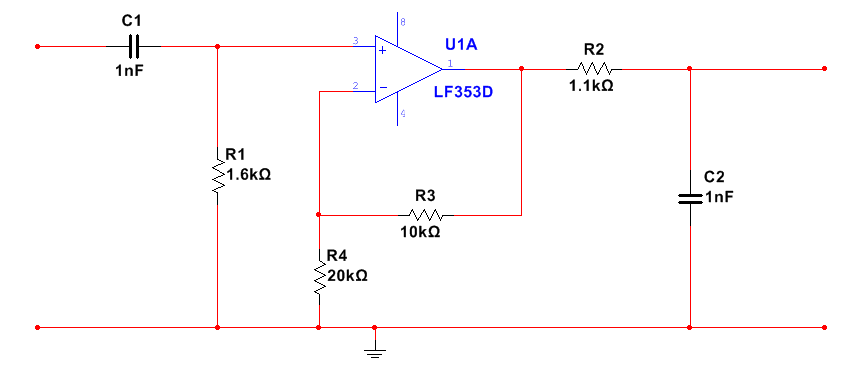
\includegraphics[width=\textwidth]{billeder/HWdesign/BAANDPAS_MV}
      \caption{Båndpasfilter med værdier}
    \label{fig:BAANDPAS_MV}
  \end{minipage}
  \hspace{0.1\textwidth}
  \begin{minipage}{0.45\textwidth}
    \centering
      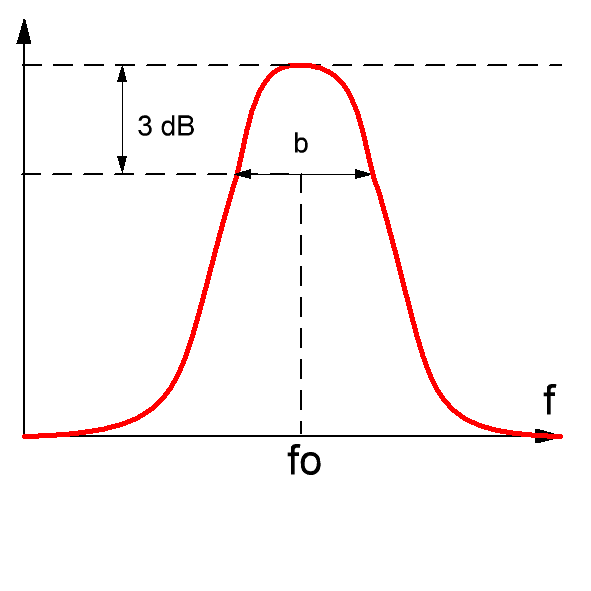
\includegraphics[width=\textwidth]{billeder/HWdesign/BAANDPAS_KURVE}
      \caption{Kurvekarakteristik for båndpasfilter}
    \label{fig:BAANDPAS_KURVE}
  \end{minipage}
\end{figure}

Båndpasfilteret har til opgave at filtrere alle signaler med frekvenser over og under 120 kHZ fra samtidig med at det forstærker signalet i båndpasset. Forstærkningen opnås ved at koble en ikke inverterende OpAmp med modstande, hvis størrelse afhænger af den ønskede forstærkning, mellem et højpasfilter og lavpasfilter som illustreret på figur \ref{fig:BAANDPAS_UV}. Kurvekarakteristikken er illustreret på figur \ref{fig:BAANDPAS_KURVE}.

Da vi ønsker at forstærke 120 kHz signalet, designes højpasfilteret således at knækfrekvensen udregnes til 110 kHz, og for lavpasfilteret beregnes en knækfrekvens på 130 kHz.

\subsection{Envelope Detector}

\begin{figure}[htbp]
	\centering
	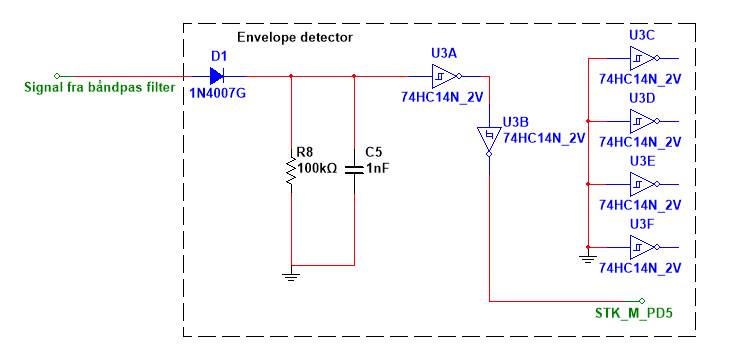
\includegraphics[width=0.70\textwidth]{billeder/HWdesign/ED_MV.png}
	\caption{Envelope detector}
	\label{fig:ED_MV}
\end{figure}

Envelope detectorens opgave er at udglatte burstsignalet fra båndpasfilteret og lave det om til et TTL (0-5V) signal som STK-kitten kan aflæse.

Den er opbygget af en diode, et RC-led og en schmitt trigger. Dioden har til opgave at sortere alle de negative halvperioder fra og kun sende de positive halvperioder til RC-leddet. Kondensatoren vil derfor kun opfange de positive halvperioder, og undgå at belaste det foranliggende kredsløb ved at aflade de negative halvperioder. Kondensatoren er med til at udglatte signalet da den ikke kan nå at aflades på en periode.

Modstanden $R_8$ er en afladningsmodstand, og den bestemmer hvor hurtigt kredsløbet skal aflades, jo højere modstand jo langsommere går det med at aflade.

Der er anvendt en schmitt trigger til at lave signalet om til et firkantet signal som STK-kitten kan aflæses. Grunden til at der er brugt 2 er fordi de er inverterende.
\newpage

